\section{Halbleiter}
\subsection{pn-Übergang}
  \begin{minipage}{14cm}
    N-Schicht wird mit Phosphor dotiert, dadurch entsteht ein Elektron welches schwächer gebunden ist.
    P-Schicht wird mit Bor dotiert, dadurch hat ein Si-Atom eine unaufgefüllte Schale. \\ \\
    Durch Anlegen einer \textbf{positiven} Spannung an der P-Zone, wird die Raumladungszone (RLZ) schmaler. 
    Dadurch wird der pn-Übergang leitend.\\
    Durch Anlegen einer \textbf{negativen} Spannung an der P-Zone, wird die Raumladungszone breiter. 
    Der pn-Übergang sperrt.
  \end{minipage}
  \begin{minipage}{5cm}
    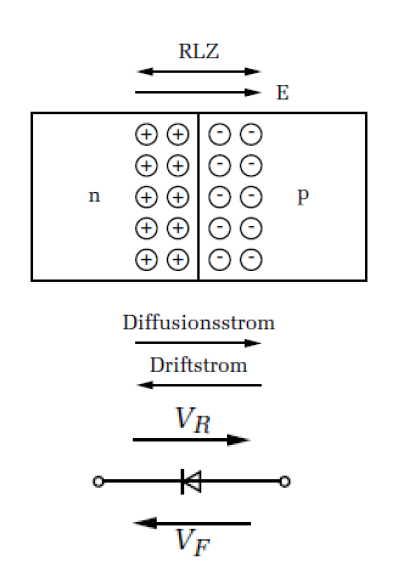
\includegraphics[width=5cm]{./bilder/pn_uebergang.png}
  \end{minipage}

\subsection{Diode}
  \underline{\bf Temperaturverhalten}\\
  Thermospannung
  \hspace{15.3mm}\fbox{$V_T = \frac{k_B\cdot T}{q}$} $V_{T_{23^\circ C}} = 25.5 mV$ \fbox{$k_B=1.38065 \cdot 10^{-23}$ J/K; $q=1.6021765 \cdot 10^  {-19}$ C; $T$=Temp [K]}\\
  \begin{minipage}[T]{8cm}
    {\bf Sperrbetrieb}\\
    $U_{np} > 5.7V$: Temp-Koeff: $+2 mV/K$\\
    $U_{np} < 5.7V$: Temp-Koeff: $-0.5 mV/K$\\
  \end{minipage}
  \begin{minipage}{5cm}
    {\bf Durchlassbetrieb}\\
    Temp-Koeff: $-2 mV/K$\\
    typisch $U_{F0} = 0.6V$
  \end{minipage}
  \begin{minipage}{6cm}
    Verdoppelung des Sperrstroms bei einer Temperaturerhöhung von $10^\circ C$
  \end{minipage}
            
  \underline{\bf Strom-Spannungs-Verhalten}\\
  \begin{minipage}[T]{8.5cm}
    Vorw\"artsstrom $I_f$
    \hspace{14.6mm}\fbox{$I_f = I_S\cdot \left(e^\frac{V_f}{m\cdot V_T} -1\right)$}\\
  \end{minipage}
  \begin{minipage}{7cm}
    $I_S$=S\"attigungssperrstrom ($<$ pA)\\
    $m$= Emissionskoeff. ($1<m<2$, meist ca. 1)\\
    $V_T$=Thermospannung
  \end{minipage}
  \begin{minipage}{3.5cm}
    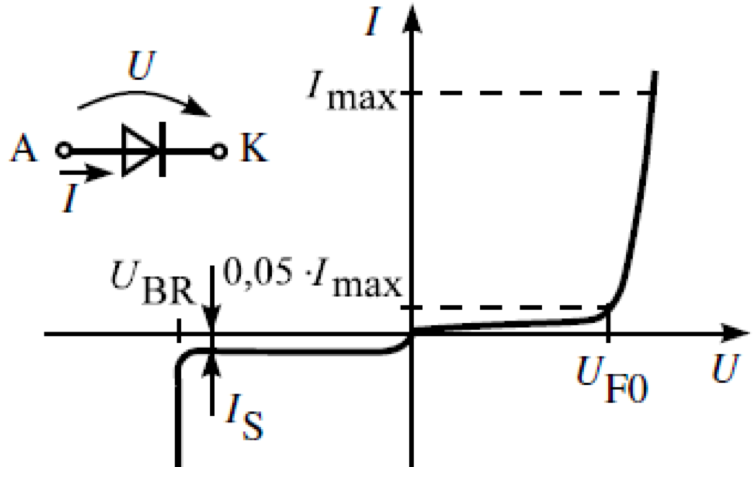
\includegraphics[width=3.5cm]{./bilder/IU_Kennlinie_Diode}\\
  \end{minipage}
  gilt für $V_f \leq U_{F0}$ (sperrend). Für $V_f \geq U_{F0}$ ist die Kurve linear (leitend).\\

  \begin{minipage}[T]{9.5cm}
    Sperrstrom $I_{SP}$
    \hspace{18mm}\fbox{$I_{SP}(T) = I_{SP}(T_0)\cdot e^{C_R\cdot(T-T_0)}$}\\
    temperaturabh\"angig
    \hspace{11mm}\fbox{$C_{R_{Si}} = \frac{W_g}{2\cdot k_B\cdot T_0^2} \cong 0.07 K^{-1}$}\\
  \end{minipage}
  \begin{minipage}{6cm}
    $T_0 = 300K$\\
    $C_{R_{Si}}$ (f\"ur Silizium bei Raumtemp.)\\
    $W_g$ Energie
  \end{minipage}
  \begin{minipage}{3.5cm}
    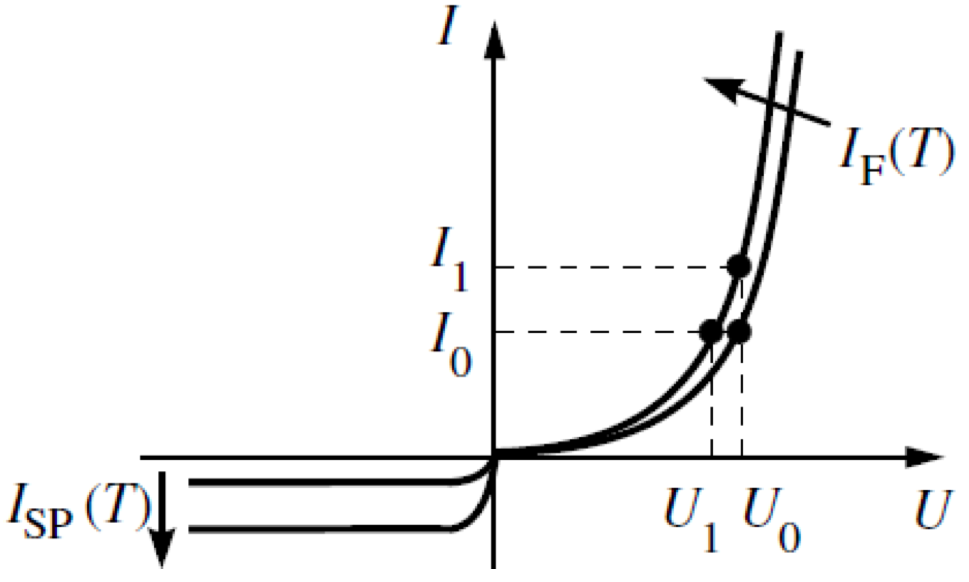
\includegraphics[width=3.5cm]{./bilder/IspKennlinieDiodeTemp}\\
  \end{minipage}\\
  {\bf Faustregel:} Verdoppelung des Sperrstroms bei einer Temperaturerh\"ohung um $10 ^\circ C$
            
  \begin{minipage}[T]{8.5cm}
    Grosssignalwiderstand
    \hspace{8mm}\fbox{$R_D = \frac{V_0}{I_0}$}\\
    Kleinsignalwiderstand
    \hspace{8.4mm}\fbox{$r_d = \frac{mV_T}{I_0} = \frac{dV}{dI}$}\\
  \end{minipage}
  \begin{minipage}{5cm}
    $V_0$= Arbeitspunkt-Spannung\\
    $I_0$= Arbeitspunkt-Strom\\
    $V_T$=Thermospannung
  \end{minipage}
  \begin{minipage}{5.5cm}
    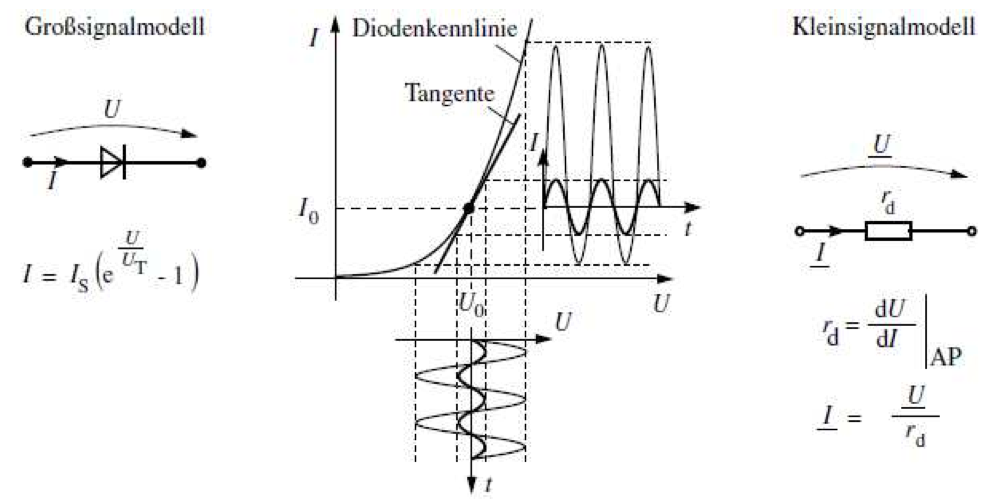
\includegraphics[width=5.5cm]{./bilder/GrossKleinSig}\\
  \end{minipage}
  
        

  \begin{minipage}[T]{15.5cm}
    \underline{\bf Kleinsignalersatzschaltbild}\\
    $R_B$: Bahnwiderstand (Zuleitung, Kontaktierung) : gerader Verlauf der Kennlinie ab $U_f >0.6V$\\
    $r_d$: differentieller Widerstand des pn-\"Ubergangs\\
    $C_D$: Diffusionskapazit\"at bei positiver Diodenspannung\\
    $C_S$: Sperrschichtkapazit\"at bei negativer Diodenspannung\\
  \end{minipage}
  \begin{minipage}{3.5cm}
    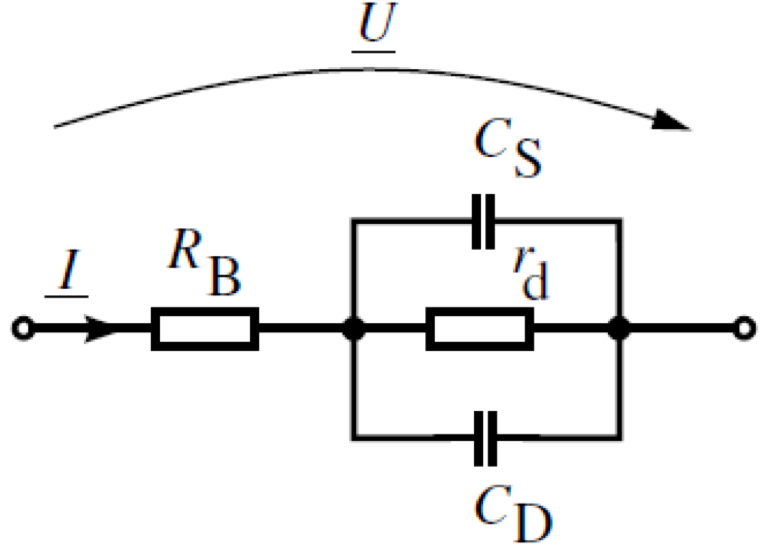
\includegraphics[width=3.5cm]{./bilder/DiodeKleinsigErs}\\
  \end{minipage}\\
  
  \hrule
  \vspace{1mm}
   \begin{minipage}[t]{9cm}
    \underline{\bf Zener-Diode}\\
    $I_{Z0} \approx 0.05 \cdot I_{Zmax}$\\
    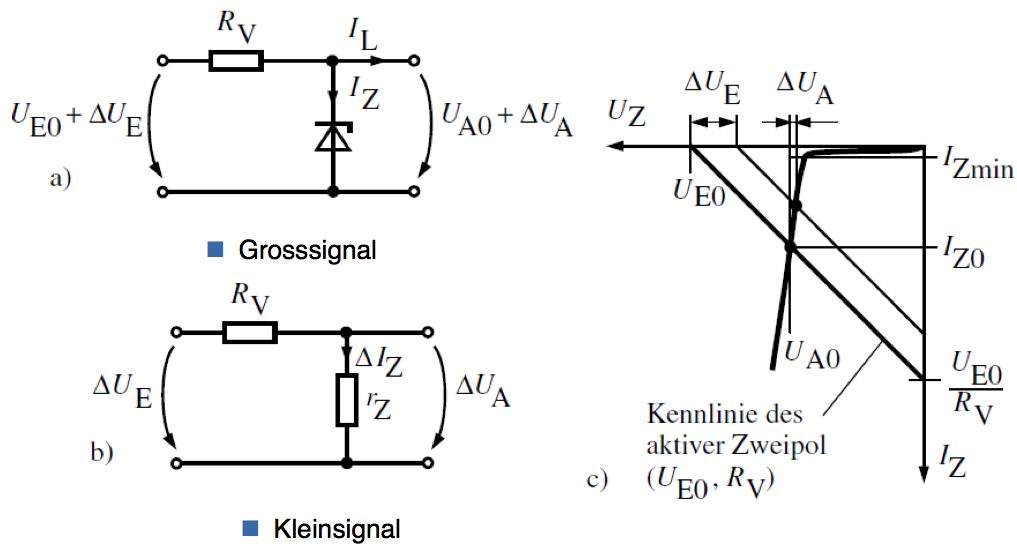
\includegraphics[height=4cm]{./bilder/ZDiodeEig} 
  \end{minipage}
  \begin{minipage}[t]{9cm}
    \underline{\bf Kapazit\"atsdiode (Varicap)}\\
    \begin{minipage}[t]{4.9cm}
      \fbox{$C_S = C_{S0} \cdot\left(1+ \frac{U_{SP}}{U_D}\right)^{-q}$}\\\\
      $q \cong 0.5$\\
      $U_{SP}$: gew\"ahlte Sperrspannung\\
      $C_S$: resultierende Kapazit\"at
    \end{minipage}
    \begin{minipage}{4cm}
      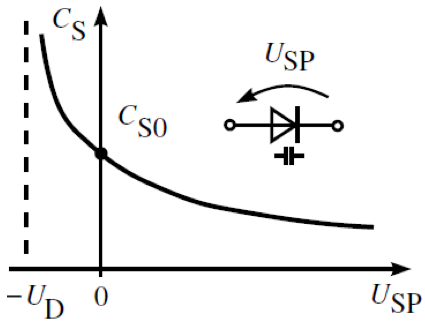
\includegraphics[width=4cm]{./bilder/CDiodeEig}
    \end{minipage}
  \end{minipage}\\
  
\hrule
